\chapter{Sampling and Data Collection}
\chaplabel{data}

\section{Introduction}
This chapter introduces students to the concepts of Analog-to-Digital Converters (ADCs) and data collection.

\section{Sampling}

The real world has signals that are continuous in both time and amplitude. Unfortunately, microcontrollers 
do not have continuous time or amplitude capabilities. This means that real signals have to be quantized 
in amplitude and sampled in time before they can be analyzed by a microcontroller. Figure \ref{fig:quantized}
shows what quantization in amplitude looks like. The microcontroller can only see values of -3 to +3 in 
this example even though the real signal has values between these. Figure \ref{fig:quantizederror} 
includes the errors incurred due to quantization.

\begin{figure}[!htb]
	\centering
	\includegraphics[scale=0.5]{dataCollection/quantized.eps}
	\caption{This shows amplitude quantization.}
	\label{fig:quantized}
\end{figure}

\begin{figure}[!htb]
	\centering
	\includegraphics[scale=0.5]{dataCollection/quantizedError.eps}
	\caption{This shows amplitude quantization and the resulting error.}
	\label{fig:quantizederror}
\end{figure}

Sampling in the time domain could be done in a random fashion as demonstrated in Figure \ref{fig:randsample}
but that is rarely a good idea. The math that can be done with a signal that is sampled at an even rate 
as shown in Figure \ref{fig:evensampling} is very powerful. Therefore, we try very hard to sample at 
a specific frequency with minimal jitter in the time between samples.

\begin{figure}[!htb]
	\centering
	\includegraphics[scale=0.5]{dataCollection/randomSampling.eps}
	\caption{This shows random sampling.}
	\label{fig:randsample}
\end{figure}

\begin{figure}[!htb]
	\centering
	\includegraphics[scale=0.5]{dataCollection/evenSampling.eps}
	\caption{This shows even sampling.}
	\label{fig:evensampling}
\end{figure}

A signal that has been both quantized and sampled is shown in Figure \ref{fig:samplequantized}. The 
signal has been reduced to the sequence of numbers: \{0,3,3,0,-3,-2\}.

\begin{figure}[!htb]
	\centering
	\includegraphics[scale=0.5]{dataCollection/sampledAndQuantized.eps}
	\caption{This shows a sampled and quantized signal.}
	\label{fig:samplequantized}
\end{figure}

It is important to sample fast enough to actually capture the signal of interest. The minimum 
sampling rate to capture a particular signal is called the  
\href{https://en.wikipedia.org/wiki/Nyquist_frequency}{Nyquist rate or Nyquist frequency}. The 
sampling rate for a signal must be at least twice the highest frequency in the signal in order 
to correctly see the signal in a sampled system. Figure \ref{fig:nyquist1} shows the best case 
when sampling at exactly twice the frequency of the signal. This can be noted since there are 
two sample points in one period of the sine wave. The worst case of sampling at exactly the 
Nyquist rate is shown in Figure \ref{fig:nyquist2}. A zoomed out version is shown in 
Figure~\ref{fig:nyquist3}. This is why it is best to give a little overhead when choosing 
the sample rate to use on a signal. If that is done, it yields Figure~\ref{fig:nyquist4} where 
the sampling rate is just a little over the frequency of the sine wave.

\begin{figure}[!htb]
	\centering
	\includegraphics[scale=0.5]{dataCollection/nyquist1.eps}
	\caption{This is the best case when sampling at the Nyquist rate.}
	\label{fig:nyquist1}
\end{figure}

\begin{figure}[!htb]
	\centering
	\includegraphics[scale=0.5]{dataCollection/nyquist2.eps}
	\caption{This is the worst case when sampling at exactly the Nyquist rate.}
	\label{fig:nyquist2}
\end{figure}

\begin{figure}[!htb]
	\centering
	\includegraphics[scale=0.5]{dataCollection/nyquist3.eps}
	\caption{This is a zoomed out view of the worst case of sampling at exactly the Nyquist rate.}
	\label{fig:nyquist3}
\end{figure}

\begin{figure}[!htb]
	\centering
	\includegraphics[scale=0.5]{dataCollection/nyquist4.eps}
	\caption{This is a zoomed out view of sampling just faster than the Nyquist rate.}
	\label{fig:nyquist4}
\end{figure}

In order to make sure that the signal never has too high frequencies, a circuit designer
will typically have a low pass filter just before the input to the ADC.

\section{ADCs}
Analog-to-digital converters (ADCs) are the piece of equipment that samples and quantizes a real signal.
They have a set bit width. For instance a 10-bit ADC returns quantized values between 0 and 1023. Setting
the sample rate can be done different ways depending on what the hardware capabilities are. Some ADCs 
take care of the sampling timing while others require the microcontroller to send a start conversion 
signal every time a new sample needs to be taken.

Once a sample is collected, it is often useful to convert it back into the voltage from the ADC count 
returned to the microcontroller. Equation \ref{eq:adc2volt} shows how this is done. The reference 
voltage is set somewhere in the system. It is a carefully constructed power supply to have as little
noise as possible. In the case of the Arduino Nano Connect RP2040, the onboard ADC reference is 3.3~V.
The onboard ADCs are also 10-bit, so if an ADC reads 400 the applied voltage is 1.29~volts as shown in 
Equation~\ref{eq:adc2voltex}. It can also be useful to know how many volts each count of the ADC is. 
This is shown in Equation~\ref{eq:adcpercount} which gives 3.222~mV per count on the Nano's ADC.

\begin{equation}
	\label{eq:adc2volt}
	\mathrm{voltage} = \left(\frac{\mathrm{ADCcount}}{\mathrm{maxADCcount}}\right)\mathrm{referenceVoltage}
\end{equation}

\begin{equation}
	\label{eq:adc2voltex}
	\mathrm{voltage} = \left(\frac{400}{1024}\right)3.3 = 1.29\mathrm{V}
\end{equation}

\begin{equation}
	\label{eq:adcpercount}
	\mathrm{volts/count} = \frac{referenceVoltage}{maxADCcount} = \frac{3.3}{1024} = 3.222\mathrm{mV}/\mathrm{count}
\end{equation}


\section{Data Collection}

\subsection{Why Do We Collect Data?}
One reason we collect data is to document something. It is important to record what has happened. One example of this 
is weather data that has been collected for centuries. This documentation then allows for analysis (another reason to 
collect data). Analysis of weather data over time led to 

\subsection{How Can We Tell If Data is Good?}

\subsection{Examples}

\section{Laboratory Exercises}
\subsection{To Do}
For the lab, collect the following data and display it once a second on the display with the 
appropriate units if you can make them fit.
\begin{enumerate}
	\item The output from \lstinline@millis()@ (ms)
	\item Light intensity as a number between 0 and 1023 (unitless)
	\item Potentiometer value as a voltage between 0 and 3.3~V
	\item Battery voltage as a voltage between 0 and 6.6~V
	\item Temperature in Fahrenheit
	\item Relative humidity in \%
	\item Distance as a number (unitless)
	\item Color as integers between 0 and 255 in the form (R,G,B) (unitless)
	\item Accelerometer readings in g's (ax, ay, az) (g)
	\item Gyroscope readings in degrees per second (gx, gy, gz) (dps)
\end{enumerate}

\subsection{Suggestions}
Do the temperature and humidity last since the SHT31 sensor sometimes requires power cycling 
to get working after uploading code to the Nano Connect.

Use a \href{https://www.arduino.cc/reference/en/language/variables/data-types/stringobject/}{String} 
object to accumulate your display string and then call \lstinline@display.println(yourString)@ 
to display it. Note a few things:
\begin{enumerate}
	\item The String type starts with a capital S.
	\item You can add to the String object using \lstinline@+=@ or just \lstinline@+@, 
		but with only the plus operator, all arguments have to be of the same type. 
	\item The String object also allows you to limit the number of decimal places for \lstinline@float@ types. 
\end{enumerate}
An example is shown in Listing \ref{lst:dispstr}.
\begin{lstlisting}[caption={This is an example of using a String 
		object to display text and float variables. The floats are 
		limited to 1 decimal place such that 7.123 would be displayed as 7.1.},
		label={lst:dispstr},language=C++]
	String dispStr;
	dispStr = "T(F),H(%): ";
	dispStr += String(tF,1);
	dispStr += ",";
	dispStr += String(humidity,1);
	dispStr += "\n";
	// Control the display  
	display.clearDisplay();
	display.setTextSize(1);  // Normal 1:1 pixel scale
	display.setCursor(0,0);  // Start at top-left corner
	display.println(dispStr);
	display.display();
\end{lstlisting}

\subsection{Turn In}
Submit a copy of your code and a video (or link to a video) of your board running your code. The 
video should include both lab partners faces.